% =============================================================
% EK A: Sayı Sistemleri ve Kodlama
% =============================================================
\chapter{Sayı Sistemleri ve Kodlama}
\label{ch:sayi-sistemleri}
\bolumfoto[İnsanlığın bilinen en eski yapısı olan Göbekli Tepe, uygarlığın başlangıç noktasıdır. Sayı sistemleri de bilgisayar biliminin başlangıç noktasıdır: her şey ikilik tabanda bir sayıyla başlar.]{gorseller/ekA-gobeklitepe.jpg}{Göbekli Tepe -- Şanlıurfa}

\begin{tcolorbox}[
    colback=blokyesil!15,
    colframe=sinyalyesil!60!black,
    title={\textbf{Öğrenme Hedefleri}},
    fonttitle=\bfseries,
    rounded corners,
    boxrule=0.8pt
]
Bu eki tamamladığınızda aşağıdakileri yapabileceksiniz:
\begin{itemize}[nosep, leftmargin=*]
    \item İkilik, sekizlik ve on altılık tabanlar arasında dönüşüm yapmak.
    \item İkilik tabanda toplama, çıkarma ve çarpma işlemlerini elle gerçekleştirmek.
    \item İşaret-büyüklük, bire tümleyen ve ikiye tümleyen gösterimlerini karşılaştırmak.
    \item Bir sayının ikiye tümleyen gösterimini bulmak ve taşma koşullarını belirlemek.
    \item Gray kodunun yapısını ve kullanım alanlarını açıklamak.
    \item İKO (BCD) gösterimini ve onluk tabanlı aritmetikteki rolünü tanımlamak.
    \item ASCII ve Unicode karakter kodlama standartlarını açıklamak.
    \item IEEE~754 kayan nokta gösteriminde bir sayıyı bileşenlerine ayırmak ve geri birleştirmek.
\end{itemize}
\end{tcolorbox}

Bu ekte, bilgisayar mimarisinin temelini oluşturan sayı sistemleri ve kodlama yöntemleri ele alınmaktadır. İkilik taban, taban dönüşümleri, işaretli sayı gösterimleri ve karakter kodlama gibi konular, kitabın ana bölümlerinde sıkça başvurulan ön bilgileri oluşturur.

% =====================================================
\section{İkilik Tabanda İşlemler}
\label{sec:ikilik-taban}

Günlük hayatta 10'luk tabanı kullanırız çünkü on ayrı rakamımız (0--9) vardır. İkilik taban\index{ikilik taban} ise yalnızca iki rakamdan (0 ve 1) oluşur. Bu tabanda ``2'' rakamı yoktur; tıpkı 10'luk tabanda ``10'' diye tek bir rakam olmadığı gibi. Sayısal devrelerin doğal dili ikilik taban olduğu için bilgisayar mimarisinin temelini oluşturur.

\subsection{Taban Değiştirme İşlemleri}

Değişik sayı tabanlarında gösterilen sayıları 10'luk tabana çevirmek için, her basamağın konum değerini hesaplamaya dayanan çözümleme yöntemi kullanılır. $t$ tabanında $n$ basamaklı bir sayının değeri:
\begin{equation}
(b_{n-1}\, b_{n-2}\, \ldots\, b_1\, b_0)_t = \sum_{i=0}^{n-1} b_i \times t^i
\label{eq:taban-donusum}
\end{equation}
Burada $b_i$, sağdan $i$.~basamaktaki rakamı gösterir ($b_0$ en sağdaki basamaktır).

İkilik tabanda $t = 2$ olduğu için, her basamaktaki bit ikinin ilgili kuvveti ile çarpılır ve sonuçlar toplanır.

\begin{ornek}[A.1]
İkilik tabandaki $1010011$ sayısını 10'luk tabana çevirin.

\textbf{Çözüm:}
\begin{align*}
(1010011)_2 &= 1\times 2^6 + 0\times 2^5 + 1\times 2^4 + 0\times 2^3 + 0\times 2^2 + 1\times 2^1 + 1\times 2^0 \\
&= 64 + 0 + 16 + 0 + 0 + 2 + 1 \\
&= (83)_{10}
\end{align*}
\end{ornek}

\begin{ornek}[A.2]
İkilik tabandaki $100101010$ sayısının 10'luk tabanda değeri nedir?

\textbf{Çözüm:}
\begin{align*}
(100101010)_2 &= 1\times 2^8 + 0\times 2^7 + 0\times 2^6 + 1\times 2^5 + 0\times 2^4 + 1\times 2^3 + 0\times 2^2 + 1\times 2^1 + 0\times 2^0 \\
&= 256 + 32 + 8 + 2 \\
&= (298)_{10}
\end{align*}
\end{ornek}

Sayılar onluk tabandan ikilik tabana çevrilmek istendiğinde, sayının içerisinde ikinin üssü olabilecek değerler aranır. Sayıdan küçük ve ikinin üzeri olan en büyük değer bulunduğunda, sonuçta ortaya çıkacak ikilik tabandaki sayının ilgili basamağına 1 değeri verilir ve sayıdan ikinin üssü olarak bulunan değer çıkarılır. Bu işlem tüm basamaklar için yinelenir.

\begin{ornek}[A.3]
$(83)_{10}$ sayısını çıkarma yöntemini kullanarak ikilik tabana çevirin.

\textbf{Çözüm:}

\begin{table}[H]
\centering
\begin{tabular}{ll}
\toprule
\textbf{İşlem Adımı} & \textbf{İkilik Tabandaki Sayı} \\
\midrule
$(83)_{10} - 2^6 = 19$ & 1 \\
$19 < 2^5$ & 10 \\
$19 - 2^4 = 3$ & 101 \\
$3 < 2^3$ & 1010 \\
$3 < 2^2$ & 10100 \\
$3 - 2^1 = 1$ & 101001 \\
$1 - 2^0 = 0$ & 1010011 \\
\bottomrule
\end{tabular}
\end{table}
\end{ornek}

Onluk tabandaki bir sayıyı ikilik tabana çevirmek için sayıyı sürekli ikiye bölerek kalana bakma yöntemi de kullanılabilir.

\begin{ornek}[A.4]
$(83)_{10}$ sayısını ikiye bölme yöntemini kullanarak ikilik tabana çevirin.

\textbf{Çözüm:}

\begin{table}[H]
\centering
\begin{tabular}{ll}
\toprule
\textbf{İşlem Adımı} & \textbf{Kalan} \\
\midrule
$83 / 2 = 41$ & 1 \\
$41 / 2 = 20$ & 1 \\
$20 / 2 = 10$ & 0 \\
$10 / 2 = 5$ & 0 \\
$5 / 2 = 2$ & 1 \\
$2 / 2 = 1$ & 0, Sonuç $= 1$ \\
\bottomrule
\end{tabular}
\end{table}

Bölme işlemlerinin ardından, son bölme işleminin sonucu en büyük basamağı ve bölme işlemlerinin kalanları diğer basamakları oluşturacak biçimde kalanlar sırayla yazılır ve sonuç $(83)_{10} = (1010011)_2$ olarak bulunur.
\end{ornek}

\subsection{İkilik Tabanda Dört İşlem}

İkilik tabanda yapılan dört işlemde, onluk tabanda kullanılan tüm kurallar geçerlidir.

\subsubsection*{Toplama işlemi:} 0 ve 1 dışında bir rakam kullanılamadığı için, ikilik tabanda onluk tabandan farklı olarak, iki basamağın toplamı 1'den büyük çıktığında toplam basamağına toplamın 2'ye bölümünden kalan yazılır ve soldaki basamağa bir elde aktarılır.

\begin{ornek}[A.5]
$(1101011)_2$ sayısı ile $(11011)_2$ sayısını toplayın.

\textbf{Çözüm:}
\[
\begin{array}{r}
  1101011 \\
+ \;\; 11011 \\
\hline
10000110
\end{array}
\]
Toplama sağdan sola yapılır. İki bitin toplamı 2'ye ulaştığında ($1+1=10$) o basamağa 0 yazılır ve soldaki basamağa bir elde aktarılır. En soldaki basamaktan taşan elde, sonucun sekizinci bitini oluşturur.
\end{ornek}

\subsubsection*{Çıkarma işlemi:} Onluk tabandan farklı olarak, elde alınacak olan yan basamaktan 10 yerine 2 alınır.

\begin{ornek}[A.6]
$(1101011)_2$ sayısından $(11011)_2$ sayısını çıkarın.

\textbf{Çözüm:}
\[
\begin{array}{r}
1101011 \\
- \;\; 11011 \\
\hline
1010000
\end{array}
\]
Çıkarma sağdan sola yapılır. Bir basamakta çıkarılan bit daha büyükse, soldaki basamaktan 2 borç alınır (onluk tabandaki 10 borç almaya karşılık gelir).
\end{ornek}

Bilgisayar donanımında çıkarma işlemi genellikle ayrı bir devre ile yapılmaz. Bunun yerine çıkarılacak sayının ikiye tümleyeni alınır ve toplama devresi kullanılır: $A - B = A + (-B)$. Bu sayede tek bir toplayıcı devresi hem toplama hem de çıkarma işlemini gerçekleştirebilir (bkz.\ Ek~\ref{ch:sayisal-tasarim}).

\subsubsection*{Çarpma işlemi:} İkilik tabandaki çarpma işleminde, ara çarpımların toplanması sırasında ikilik tabanda yapılan toplama işleminin kuralları uygulanır.

\begin{ornek}[A.7]
$(1101)_2$ sayısı ile $(11)_2$ sayısını çarpın.

\textbf{Çözüm:}
\[
\begin{array}{r}
1101 \\
\times \;\; 11 \\
\hline
1101 \\
1101\phantom{0} \\
\hline
100111
\end{array}
\]
\end{ornek}

\subsubsection*{Bölme işlemi:} İkilik tabanda, çarpma ve çıkarma işlemlerindeki kurallar gözetilerek bölme işlemi yapılmaktadır.

\begin{ornek}[A.8]
$(110101)_2$ sayısını $(110)_2$ sayısına bölün.

\textbf{Çözüm:}

Onluk bölmedeki gibi, bölünenin solundaki basamaklardan başlanır. Bölen sığıyorsa bölüm basamağına 1, sığmıyorsa 0 yazılır:
\begin{itemize}[nosep]
    \item İlk 3 bit $(110)$: bölen $110$'a eşit $\Rightarrow$ bölüm biti $= 1$, kalan $= 000$.
    \item Sonraki bit indirilir: $0001 < 110$ $\Rightarrow$ bölüm biti $= 0$.
    \item Sonraki bit indirilir: $00010 < 110$ $\Rightarrow$ bölüm biti $= 0$.
    \item Son bit indirilir: $000101 < 110$ $\Rightarrow$ bölüm biti $= 0$.
\end{itemize}
\[
(110101)_2 \div (110)_2 = (1000)_2 \quad \text{kalan: } (101)_2
\]
Doğrulama: $(53)_{10} \div (6)_{10} = (8)_{10}$, kalan $(5)_{10}$.
\end{ornek}


\subsection{8'lik ve 16'lık Tabanda İşlemler}

Onluk tabanda kullanılan sayılar ikilik tabanda gösterilirken, onluk tabandaki sayı büyüdükçe, ikilik tabandaki sayının basamak sayısı hızla artar. İkilik tabanda yalnızca iki rakam olduğu için, ortaya çıkan bu basamak sayısı fazla sayıların programcı tarafından yazılması, okunması ve takip edilmesi zordur. Bu nedenle bilgisayarlarda çalıştırılacak çevirici dil kodlarının yazımında kolaylık sağlaması amacıyla sayılar 8'lik\index{sekizlik taban} ya da 16'lık\index{on altılık taban} sayı tabanlarında gösterilir.

$8 = 2^3$ ve $16 = 2^4$ olduğu için, ikilik tabanda yazılmış bir sayıyı 8'lik tabana (İngilizcesi: \textit{octal}) çevirmek için sayının basamaklarını üçerli, 16'lık tabana (İngilizcesi: \textit{hexadecimal}) çevirmek için de sayının basamaklarını dörderli gruplamak gerekir. Tablo~\ref{tab:hex-tablo}'de 16'lık tabandaki her basamağın 10'luk, 8'lik ve 2'lik tabanlardaki karşılıkları verilmiştir.

\begin{table}[H]
\centering
\caption{16'lık tabandaki sayıların diğer tabanlardaki gösterimleri}
\label{tab:hex-tablo}
\begin{tabular}{cccc}
\toprule
\textbf{16'lık} & \textbf{10'luk} & \textbf{8'lik} & \textbf{2'lik} \\
\midrule
0 & 0  & 0  & 0000 \\
1 & 1  & 1  & 0001 \\
2 & 2  & 2  & 0010 \\
3 & 3  & 3  & 0011 \\
4 & 4  & 4  & 0100 \\
5 & 5  & 5  & 0101 \\
6 & 6  & 6  & 0110 \\
7 & 7  & 7  & 0111 \\
8 & 8  & 10 & 1000 \\
9 & 9  & 11 & 1001 \\
A & 10 & 12 & 1010 \\
B & 11 & 13 & 1011 \\
C & 12 & 14 & 1100 \\
D & 13 & 15 & 1101 \\
E & 14 & 16 & 1110 \\
F & 15 & 17 & 1111 \\
\bottomrule
\end{tabular}
\end{table}

\begin{ornek}[A.9]
Onluk tabandaki $1.223.357$ sayısını ikilik, sekizlik ve onaltılık tabanda gösterin.

\textbf{Çözüm:}

İkiye bölme yöntemiyle (bkz.\ Örnek~A.4) sayı ikilik tabana çevrilir:

$(1.223.357)_{10} = (100\;101\;010\;101\;010\;111\;101)_2$

Sekizlik tabana çevirmek için basamaklar üçerli gruplanır:
\[
\underbrace{100}_{4}\;\underbrace{101}_{5}\;\underbrace{010}_{2}\;\underbrace{101}_{5}\;\underbrace{010}_{2}\;\underbrace{111}_{7}\;\underbrace{101}_{5} \implies (4525275)_8
\]

Onaltılık tabana çevirmek için basamaklar dörderli gruplanır:
\[
\underbrace{0001}_{1}\;\underbrace{0010}_{2}\;\underbrace{1010}_{A}\;\underbrace{1010}_{A}\;\underbrace{1011}_{B}\;\underbrace{1101}_{D} \implies (12AABD)_{16}
\]
\end{ornek}


% =====================================================
\section{İşaretli Sayılar}
\label{sec:isaretli-sayilar}

Şimdiye kadar hep sıfır ve pozitif sayılarla çalıştık. Peki ya eksi sayıları nasıl göstereceğiz? Bellekte saklanan bir bit dizisinin ``pozitif mi, negatif mi'' olduğunu donanım kendiliğinden bilemez; bu tamamen programcının ya da derleyicinin tercihine bağlıdır. Aynı bit dizisi, kullanılan buyruğa göre hem işaretli hem de işaretsiz bir sayı olarak yorumlanabilir.

Eksi sayıları ikilik tabanda göstermek için tarih boyunca birçok yöntem önerilmiştir. Bu yöntemlerin ortak noktası, sayının en soldaki bitini (en anlamlı bit) işaret bilgisi için ayırmaktır: bu bit 1 ise sayı eksi, 0 ise artı kabul edilir. Tablo~\ref{tab:isaretli-yontemler}'de dört farklı yöntemle 4 bitlik gösterimler karşılaştırmalı olarak verilmiştir.

\subsection{Ayrı İşaret Biti}
\index{ayrı işaret biti}

Bir sayının işaretini göstermenin en kolay yolu saklama alanının bir bitini işaret bilgisini tutmak için ayırmaktır. Ayrı işaret biti kullanan sistemlerde sayının en soldaki, en anlamlı bitinin (İngilizcesi: \textit{most significant bit -- msb}) işaret biti olduğu kabul edilir. Bu işaret bitinin değeri eğer sayı eksi ise 1, artı ise 0 olarak belirlenir.

Ayrı işaret biti kullanma yönteminde işaret biti sayıya dahil değildir ve ayrıca işlenir. Bu yöntemde $+0$ ve $-0$ olmak üzere iki ayrı sıfır değeri ortaya çıkar.

\subsection{Artık N}
\index{artık-N gösterimi}

Artık-N (İngilizcesi: \textit{Excess-N}) gösteriminde sayılara belirli bir $N$ sayısı eklenir ve sayı bu ekleme işleminin ardından ikilik tabana çevrilir. Örneğin, artık-3'te 0 sayısının nasıl gösterildiğini bulmak için önce sayıya 3 eklenir ve çıkan sonuç ikilik tabana çevrilerek $0011$ bulunur. Bu yöntemin en önemli kullanım alanı IEEE~754 kayan nokta standardında üs alanının kodlanmasıdır (bkz.\ Bölüm~\ref{sec:ekA-ieee754}). Artık-N gösteriminin avantajı, saklanan değerlerin doğrudan büyüklük karşılaştırmasına olanak tanımasıdır: saklanan bit dizileri üzerinde işaretsiz karşılaştırma yapmak, gerçek üs değerlerini karşılaştırmakla eşdeğerdir.

\begin{ornek}[A.10]
4 bitlik artık-3 gösteriminde $-2$ ve $+5$ sayılarını gösterin.

\textbf{Çözüm:}

Artık-3 gösteriminde her sayıya 3 eklenir ve sonuç ikilik tabana çevrilir:
\begin{itemize}[nosep]
    \item $-2$: \;$-2 + 3 = 1 = (0001)_2$
    \item $+5$: \;$5 + 3 = 8 = (1000)_2$
\end{itemize}
4 bitlik artık-3 gösteriminde gösterilebilecek aralık $-3$ ile $+12$ arasıdır; $0000$ en küçük ($-3$), $1111$ en büyük ($+12$) değeri temsil eder.
\end{ornek}

\subsection{Bire Tümleyen Gösterimi}
\index{bire tümleyen}

İkilik tabandaki bir sayının bire tümleyenini almak için her bir basamaktaki rakam 0 ise 1, 1 ise 0 yapılarak sayının her biti ters çevrilir. Örneğin $10101$ sayısının bire tümleyeni $01010$'dır. Bire tümleyen gösteriminde de $+0$ ve $-0$ olmak üzere iki ayrı sıfır değeri vardır. Bu çift sıfır sorunu ve toplama işleminde ``dairesel elde'' gerektirmesi gibi dezavantajları nedeniyle bire tümleyen gösterimi günümüz bilgisayarlarında neredeyse hiç kullanılmamaktadır; yerini ikiye tümleyen almıştır.

\begin{ornek}[A.11]
8 bitlik bire tümleyen gösteriminde $-45$ sayısını gösterin.

\textbf{Çözüm:}

Önce $45$ sayısı 8 bitlik ikilik tabana çevrilir: $45 = (00101101)_2$. Bire tümleyeni almak için tüm bitler ters çevrilir:
\[
-45 = \overline{00101101} = (11010010)_2
\]
Doğrulama: Bire tümleyen düzeninde bir sayı ile tümleyeninin toplamı tüm bitleri 1 olan sayıyı verir: $00101101 + 11010010 = 11111111$ \checkmark
\end{ornek}

\subsection{İkiye Tümleyen Gösterimi}
\index{ikiye tümleyen}

Bire tümleyen yönteminde sıfır değeri için iki ayrı sayı kullanılması nedeniyle gösterilebilecek sayılardan bir tanesi israf edilmektedir. İkiye tümleyen yöntemi bu sorunu ortadan kaldırmak için tasarlanmıştır. Günümüzde kullanılan sayısal devrelerin büyük çoğunluğu ikiye tümleyen yöntemi kullanmaktadır.

Bir sayının ikiye tümleyenini almak için sayının bire tümleyeni alınır ve sonuca bir eklenir.

\begin{ornek}[A.12]
$-1$ sayısının 4 bitlik 2'ye tümleyen gösteriminde karşılığı nedir?

\textbf{Çözüm:}

$1$ sayısının 4 bitle gösterilen karşılığı $0001$'dir. Bu sayının bire tümleyeni alınıp 1 eklenerek ikiye tümleyeni bulunur:
\[
1 = (0001)_2 \rightarrow -1 = \overline{0001} + 1 = (1110)_2 + 1 = (1111)_2
\]
\end{ornek}

\begin{ornek}[A.13]
$-8$ sayısının 4 bitlik 2'ye tümleyen gösteriminde karşılığı nedir?

\textbf{Çözüm:}

$8 = (1000)_2 \rightarrow -8 = \overline{1000} + 1 = (0111)_2 + 1 = (1000)_2$

İkiye tümleyen yönteminde belirli bir bit sayısıyla gösterilebilen eksi sayıların sayısı artı sayıların sayısından bir fazladır. Bu nedenle 4 bitlik alanda $-8$ gösterilebilse de $+8$ gösterilemez. 4 bitlik alanda gösterilebilen en yüksek sayı $+7$'dir.
\end{ornek}

\begin{ornek}[A.14]
İkiye tümleyen gösteriminde değeri $(1011010)_2$ olan sayının onluk tabandaki karşılığı nedir?

\textbf{Çözüm:}

Sayının işaret biti 1 olduğu için sayı eksidir. Sayının ikiye tümleyeni alınır:
\[
\overline{1011010} + 1 = (0100101)_2 + 1 = (0100110)_2 = (38)_{10}
\]
Dolayısıyla ikiye tümleyen düzeninde $(1011010)_2 = -38$'dir.
\end{ornek}

Bir sayının ikiye tümleyenini bulmanın daha hızlı bir yolu vardır: sayının en sağdaki bitinden başla, sola doğru yürü, 1 olan ilk basamağa kadar bütün sıfırları ve ilk 1'i kopyala, sonraki bütün basamakları ters çevir.

\begin{ornek}[A.15]
İkiye tümleyen gösteriminde değeri $(1011010)_2$ olan sayının ikiye tümleyenini hızlı yolu kullanarak bulun.

\textbf{Çözüm:}

Sayının en sağdaki basamağından başlanır, sola doğru yürürken ilk 1'e kadar (ilk 1 dahil) tüm basamaklar kopyalanır, sonraki tüm bitler ters çevrilir:
\[
1011010 \xrightarrow{\text{hızlı yol}} 0100110
\]
\end{ornek}

\begin{ornek}[A.16]
$(-15122)_{10}$ sayısını 2'ye tümleyen yöntemini kullanarak 2'lik, 8'lik ve 16'lık düzenlerde yazın.

\textbf{Çözüm:}

Önce sayının mutlak değeri 2'lik tabana çevrilir:
\[
15122 = (011101100010010)_2
\]
Sayının ikiye tümleyeni alınır:
\[
(-15122)_{10} = (100010011101110)_2
\]
8'lik tabana çevirmek için 3'erli gruplara ayrılır:
\[
\underbrace{100}_{4}\;\underbrace{010}_{2}\;\underbrace{011}_{3}\;\underbrace{101}_{5}\;\underbrace{110}_{6} \implies (-15122)_{10} = (42356)_8
\]
16'lık tabana çevirmek için 4'erli gruplara ayrılır:
\[
\underbrace{1100}_{C}\;\underbrace{0100}_{4}\;\underbrace{1110}_{E}\;\underbrace{1110}_{E} \implies (-15122)_{10} = (C4EE)_{16}
\]
Eksi sayılarda 4'erli gruplara ayrılırken en soldaki grubun başına 0 değil 1 eklenir.
\end{ornek}

\begin{ornek}[A.17]
16'lık tabandaki $FC36A$ sayısını 2'lik, 8'lik ve 10'luk düzende gösterin.

\textbf{Çözüm:}

Her bir hane 4 bitlik ikilik tabana çevrilir:
\[
\underbrace{F}_{1111}\;\underbrace{C}_{1100}\;\underbrace{3}_{0011}\;\underbrace{6}_{0110}\;\underbrace{A}_{1010}
\]
\[
(FC36A)_{16} = (11111100001101101010)_2
\]
Sekizlik tabana çevirmek için 3'erli gruplara ayrılır:
\[
(FC36A)_{16} = (3741552)_8
\]
İşaretli kabul edilirse, en soldaki bit 1 olduğu için eksidir. İkiye tümleyeni alınarak:
\[
(FC36A)_{16} = -(15510)_{10} \quad \text{(işaretli)}
\]
İşaretsiz kabul edilirse:
\[
(FC36A)_{16} = (1033066)_{10} \quad \text{(işaretsiz)}
\]
\end{ornek}

\begin{table}[H]
\centering
\caption{Değişik yöntemlerde 4 bitle gösterilen sayılar}
\label{tab:isaretli-yontemler}
\begin{tabular}{ccccc}
\toprule
\textbf{İkilik} & \textbf{Ayrı İşaret} & \textbf{1'e Tümleyen} & \textbf{Artık-3} & \textbf{2'ye Tümleyen} \\
\midrule
0000 & $+0$ & $+0$ & $-3$ & $0$  \\
0001 & $1$  & $1$  & $-2$ & $1$  \\
0010 & $2$  & $2$  & $-1$ & $2$  \\
0011 & $3$  & $3$  & $0$  & $3$  \\
0100 & $4$  & $4$  & $1$  & $4$  \\
0101 & $5$  & $5$  & $2$  & $5$  \\
0110 & $6$  & $6$  & $3$  & $6$  \\
0111 & $7$  & $7$  & $4$  & $7$  \\
1000 & $-0$ & $-7$ & $5$  & $-8$ \\
1001 & $-1$ & $-6$ & $6$  & $-7$ \\
1010 & $-2$ & $-5$ & $7$  & $-6$ \\
1011 & $-3$ & $-4$ & $8$  & $-5$ \\
1100 & $-4$ & $-3$ & $9$  & $-4$ \\
1101 & $-5$ & $-2$ & $10$ & $-3$ \\
1110 & $-6$ & $-1$ & $11$ & $-2$ \\
1111 & $-7$ & $-0$ & $12$ & $-1$ \\
\bottomrule
\end{tabular}
\end{table}

İkiye tümleyen yönteminde gösterilen işaretli sayıların daha yüksek sayıda bitle ifade edilmesi gerektiğinde \textbf{İşaretle Genişletme}\index{işaretle genişletme} (İngilizcesi: \textit{Sign Extension}) kullanılır. Sayının işaret bitinin kendisinin soluna eklenmesiyle sayı daha büyük bir alana yazılabilir hale gelir. Örneğin 4 bitlik $1110$ sayısı ikiye tümleyen gösteriminde $-2$'ye karşılık gelir. 8 bite işaretle genişletilirse ortaya çıkan $11111110$ sayısının değeri de $-2$'dir.

\subsection{Taşma Tespiti}
\label{sec:tasma-tespiti}
\index{taşma}

İşaretli sayılarla aritmetik işlem yapılırken sonuç, kullanılan bit sayısının gösterebileceği aralığın dışına çıkabilir. Bu duruma \textbf{taşma}\index{taşma} (İngilizcesi: \textit{overflow}) denir. İkiye tümleyen gösteriminde $n$ bitlik bir alan $-2^{n-1}$ ile $+2^{n-1}-1$ arasındaki sayıları gösterebilir; sonuç bu aralığın dışına çıktığında taşma oluşur.

İkiye tümleyende taşma yalnızca aynı işaretli iki sayı toplandığında ortaya çıkabilir:
\begin{itemize}
    \item İki pozitif sayı toplanıp sonucun işaret biti 1 olursa (sonuç negatif görünür) $\Rightarrow$ taşma var.
    \item İki negatif sayı toplanıp sonucun işaret biti 0 olursa (sonuç pozitif görünür) $\Rightarrow$ taşma var.
    \item Farklı işaretli iki sayının toplamında taşma oluşmaz; sonucun büyüklüğü her zaman işlenenlerin büyüklüğünden küçüktür.
\end{itemize}

Taşma donanım düzeyinde en anlamlı bit konumundaki elde girişi ($c_{n-1}$) ile elde çıkışının ($c_n$) karşılaştırılmasıyla tespit edilir: $c_{n-1} \neq c_n$ ise taşma vardır.

\begin{ornek}[A.18]
4 bitlik ikiye tümleyen düzeninde $5 + 4$ işlemini yapın ve taşma olup olmadığını belirleyin.

\textbf{Çözüm:}
\[
\begin{array}{r@{\quad}l}
  0101 & (+5)\\
+\; 0100 & (+4)\\
\hline
  1001 & (-7\text{?})
\end{array}
\]
Sonuç $1001$'dir ve işaret biti 1'dir; ikiye tümleyen düzeninde bu $-7$'ye karşılık gelir. İki pozitif sayı toplanmasına karşın sonuç negatif çıktığı için taşma oluşmuştur. Gerçek sonuç olan $+9$, 4 bitlik alanda ($-8$ ile $+7$ arası) gösterilemez.
\end{ornek}

\begin{ornek}[A.19]
4 bitlik ikiye tümleyen düzeninde $(-6) + (-5)$ işlemini yapın ve taşma olup olmadığını belirleyin.

\textbf{Çözüm:}

$-6 = (1010)_2$, $-5 = (1011)_2$:
\[
\begin{array}{r@{\quad}l}
  1010 & (-6)\\
+\; 1011 & (-5)\\
\hline
\mathbf{1}\;0101 & (+5\text{?})
\end{array}
\]
Elde çıkışı atıldığında sonuç $0101$, başka bir deyişle $+5$ olarak görünür. İki negatif sayının toplamının pozitif çıkması taşma olduğunu gösterir. Gerçek sonuç olan $-11$, 4 bitlik alanda gösterilemez.
\end{ornek}

\begin{ornek}[A.20]
4 bitlik ikiye tümleyen düzeninde $3 + (-5)$ işlemini yapın ve taşma olup olmadığını belirleyin.

\textbf{Çözüm:}

$3 = (0011)_2$, $-5 = (1011)_2$:
\[
\begin{array}{r@{\quad}l}
  0011 & (+3)\\
+\; 1011 & (-5)\\
\hline
  1110 & (-2)
\end{array}
\]
Sonuç $1110$, ikiye tümleyen düzeninde $-2$'dir. Beklenen sonuç da $3 + (-5) = -2$ olduğundan taşma oluşmamıştır. Farklı işaretli iki sayının toplamında taşma asla oluşmaz; çünkü sonucun büyüklüğü her zaman işlenenlerden küçüktür.
\end{ornek}

İşaretsiz sayılarla çalışılırken ise taşma kavramı yerine \textbf{elde}\index{elde} (İngilizcesi: \textit{carry}) kavramı kullanılır. En anlamlı bitten bir elde çıkışı oluşursa sonuç $n$ bite sığmamış demektir; bu durum elde bayrağı (carry flag) ile işaretlenir. İşaretli ve işaretsiz taşmanın farklı bayraklarla izlendiğine dikkat ediniz: işlemciler genellikle hem elde (C) hem de taşma (V) bayraklarını ayrı ayrı günceller.

\begin{bilginot}[Ariane 5: Taşmanın Bedeli]
4~Haziran 1996'da Avrupa Uzay Ajansı'nın Ariane~5 roketi, fırlatılışından 37~saniye sonra yörüngeden saptı ve infilak etti. Kaza raporunda sorunun, uçuş kontrol yazılımında 64~bitlik bir kayan nokta değerinin 16~bitlik işaretli bir tam sayıya dönüştürülmesi sırasında oluşan bir taşmadan kaynaklandığı tespit edildi. Roketin yanal hız değeri 16~bitin gösterebileceği $\pm 32\,767$ aralığını aştığında yazılım kural dışı durumu tetikledi ve yedek sistem de aynı hataya düştü. Yaklaşık 370~milyon dolarlık kayıpla sonuçlanan bu olay, taşma denetiminin ne denli önemli olduğunu gösteren en çarpıcı örneklerden biridir.
\end{bilginot}

% =====================================================
\section{Gray Kodu}
\label{sec:gray-kodu}
\index{Gray kodu}

Gray Kodu, Bell Laboratuvarları'nda çalışan Frank Gray tarafından bulunmuştur. Sayıların kodlanması sırasında birbiri arasında değer açısından 1 fark olan iki sayının yalnızca 1 bitinin farklı olması esasına dayanır. Bu özellik, birden fazla bitin aynı anda değiştiği geçiş anlarında oluşabilecek hatalı ara değerleri ortadan kaldırır. Gray kodu özellikle döner konum kodlayıcılarda (rotary encoder) ve Karnaugh haritalarında (bkz.\ Ek~\ref{ch:sayisal-tasarim}) kullanılır. Tablo~\ref{tab:gray-kodu}'da 3 bitlik ikilik ve Gray kodları yan yana gösterilmiştir; ardışık satırlar arasında yalnızca tek bir bitin değiştiğine dikkat ediniz.

\begin{table}[H]
\centering
\caption{3 Bitlik Gray Kodu}
\label{tab:gray-kodu}
\begin{tabular}{ccc}
\toprule
\textbf{Onluk Taban} & \textbf{İkilik Taban} & \textbf{Gray Kodu} \\
\midrule
0 & 000 & 000 \\
1 & 001 & 001 \\
2 & 010 & 011 \\
3 & 011 & 010 \\
4 & 100 & 110 \\
5 & 101 & 111 \\
6 & 110 & 101 \\
7 & 111 & 100 \\
\bottomrule
\end{tabular}
\end{table}

İkilik tabandaki bir sayıyı Gray koduna çevirmek için basit bir kural vardır: en soldaki (en anlamlı) bit aynen korunur; sonraki her Gray biti, ikilik sayının o basamağı ile bir soldaki basamağının Dışlayan VEYA (XOR) işlemiyle elde edilir. Tersi yönde ise Gray kodundan ikilik tabana çevirirken, en soldaki bit yine aynen korunur ve sonraki her ikilik bit, bir önceki ikilik bit ile o konumdaki Gray bitinin XOR'u olarak hesaplanır.

\begin{ornek}[A.21]
$(13)_{10}$ sayısını Gray koduna çevirin.

\textbf{Çözüm:}

Önce ikilik tabana çevirelim: $13 = (1101)_2$. Şimdi XOR kuralını uygulayalım:
\[
\begin{array}{cccc}
\text{İkilik:} & 1 & 1 & 0 \quad 1 \\
& \downarrow & \downarrow\!\!\text{\small\,XOR} & \downarrow\!\!\text{\small\,XOR} \quad \downarrow\!\!\text{\small\,XOR} \\
\text{Gray:} & 1 & 0 & 1 \quad 1
\end{array}
\]
İlk bit aynen $1$; ikinci Gray biti $1 \oplus 1 = 0$; üçüncü $1 \oplus 0 = 1$; dördüncü $0 \oplus 1 = 1$. Sonuç: $(13)_{10} = (1011)_{\text{Gray}}$.
\end{ornek}


% =====================================================
\section{İkiye Kodlanmış Onluk Taban Gösterimi}
\label{sec:bcd}
\index{BCD}

Onluk tabandaki her bir rakamın ikilik tabanda kodlandığı bu gösterim biçimine \textbf{İkiye Kodlanmış Onlu} (İngilizcesi: \textit{Binary Coded Decimal -- BCD}) gösterimi denir. Onluk tabanda toplam 10 rakam vardır ve bu 10 rakam ikilik tabanda 4 bitle gösterilebilir. BCD gösteriminin özelliği 9'dan büyük bir sayı yazılacağı zaman her bir sayı basamağı için 4 bitlik rakam kodunun ayrıca kullanılmasıdır. Tablo~\ref{tab:bcd-tablo}'da 0--9 arası onluk rakamların BCD karşılıkları verilmiştir.

\begin{table}[H]
\centering
\caption{10'luk tabandaki sayıların BCD yöntemi ile gösterimleri}
\label{tab:bcd-tablo}
\begin{tabular}{cl}
\toprule
\textbf{Onluk Taban} & \textbf{BCD Gösterimi} \\
\midrule
0    & 0000 \\
1    & 0001 \\
2    & 0010 \\
3    & 0011 \\
4    & 0100 \\
5    & 0101 \\
6    & 0110 \\
7    & 0111 \\
8    & 1000 \\
9    & 1001 \\
10   & 0001 0000 \\
11   & 0001 0001 \\
154  & 0001 0101 0100 \\
1128 & 0001 0001 0010 1000 \\
\bottomrule
\end{tabular}
\end{table}

BCD gösteriminde aritmetik işlemler, olağan ikilik toplama kurallarından farklıdır. Her 4 bitlik grubun sonucu 9'u ($1001$'i) aşarsa, o gruba 6 ($0110$) eklenerek düzeltme yapılır; bu düzeltme bir elde oluşturur ve bir üst basamağa aktarılır.

\begin{ornek}[A.22]
BCD düzeninde $27 + 35$ işlemini yapın.

\textbf{Çözüm:}

Her basamağı ayrı ayrı 4 bitlik BCD olarak yazalım ve toplayalım:
\[
\begin{array}{rcl}
  & 0010\;0111 & (27)_{\text{BCD}} \\
+ & 0011\;0101 & (35)_{\text{BCD}} \\
\hline
  & 0101\;1100 &
\end{array}
\]
Alt 4 bit: $0111 + 0101 = 1100$. Bu değer $9$'dan büyük olduğu için $0110$ eklenir: $1100 + 0110 = 1\;0010$. Alt basamak $0010$ olur, bir elde yukarı aktarılır. Üst 4 bit: $0010 + 0011 + 1_{\text{elde}} = 0110$. Sonuç: $0110\;0010 = (62)_{\text{BCD}}$.
\end{ornek}


% =====================================================
\section{Karakter Kodlaması}
\label{sec:karakter-kodlama}

Bilgisayarlar sayıların yanında karakterlerle ve bu karakterlerin oluşturduğu dizgilerle de işlem yaparlar. Her ne kadar işlem yapılan veri türü bir sayı olmasa da, bilgisayarların yalnızca ikilik tabandaki 1 bitlik değerleri saklamaları nedeniyle, karakterler de ikilik tabanda sayı olarak saklanır.

\subsection{ASCII}
\label{sec:ascii}
\index{ASCII}

Ekrana basılacak harflerin ve her türlü noktalama işaretlerinin ikilik tabanda bir karşılığı olmalıdır. Dünyada en yaygın kullanılan karakter tablosu ASCII'dir\index{ASCII} (American Standard Code for Information Interchange). ASCII düzeninde her bir karakter için 7 bitlik bir kod tanımlanmıştır; bu da toplam $2^7 = 128$ farklı karakter anlamına gelir. Bu 128 kodun ilk 32'si (0--31) ve son kodu (127) denetim karakterleridir; geri kalan 95'i yazdırılabilir karakterlerdir. ASCII bellekte genellikle 1 baytlık bir alanda saklanır; kullanılmayan 8.~bit sıfır yapılır ya da eşlik denetimi için kullanılır.

İlk ortaya çıkan 128 karakterlik ASCII tablosunda Türkçe'ye özgü harfler (ç, ğ, ı, ö, ş, ü) yoktur. 1980'li yıllarda bu sorunu çözmek için 8.~bitin de kullanıldığı ``Genişletilmiş ASCII'' tabloları (128--255 arası kodlar) tanımlandı; ancak her ülke kendi tablosunu oluşturduğu için uyumsuzluklar ortaya çıktı. Türkçe için ISO~8859-9 (Latin-5) tablosu kullanılmıştır.

Şekil~\ref{fig:ascii-tablo}'de yazdırılabilir 96~ASCII karakteri (\texttt{0x20}--\texttt{0x7E} aralığı) gösterilmiştir. Tabloda satır başlığı üst yarım baytı, sütun başlığı alt yarım baytı verir; bir karakterin kodunu bulmak için satır ve sütun değerleri birleştirilir. Örneğin ``A'' harfi \texttt{4x} satırı ile \texttt{1} sütununda yer aldığı için kodu \texttt{0x41}'dir; onluk tabanda $65$'e karşılık gelir. Tablodaki ilk karakter olan SP (\textit{space}) boşluk karakterini, son karakter olan DEL ise silme denetim karakterini temsil eder.

\begin{figure}[H]
\centering
\begin{tikzpicture}[scale=1.0]
  \footnotesize\ttfamily
  % Başlık satırı
  \foreach \col [count=\ci from 0] in {0,1,2,3,4,5,6,7,8,9,A,B,C,D,E,F} {
    \node[font=\footnotesize\ttfamily\bfseries, text=vurgumavi] at (0.9*\ci+1.2, 6.8) {\col};
  }
  % Satır başlıkları (hex üst yarım bayt)
  \foreach \row/\rval in {0/2, 1/3, 2/4, 3/5, 4/6, 5/7} {
    \node[font=\footnotesize\ttfamily\bfseries, text=vurgumavi] at (0, 6.2-0.55*\row) {\rval x};
  }
  % ASCII karakterleri
  % Satır 2x (0x20-0x2F)
  \foreach \c [count=\ci from 0] in {SP,!,",\#,\$,\%,\&,',{(},{)},*,+,{,},-,.,/} {
    \node[font=\footnotesize\ttfamily] at (0.9*\ci+1.2, 6.2) {\c};
  }
  % Satır 3x (0x30-0x3F)
  \foreach \c [count=\ci from 0] in {0,1,2,3,4,5,6,7,8,9,:,;,<,=,>,?} {
    \node[font=\footnotesize\ttfamily] at (0.9*\ci+1.2, 5.65) {\c};
  }
  % Satır 4x (0x40-0x4F)
  \foreach \c [count=\ci from 0] in {@,A,B,C,D,E,F,G,H,I,J,K,L,M,N,O} {
    \node[font=\footnotesize\ttfamily] at (0.9*\ci+1.2, 5.1) {\c};
  }
  % Satır 5x (0x50-0x5F)
  \foreach \c [count=\ci from 0] in {P,Q,R,S,T,U,V,W,X,Y,Z,[,\textbackslash,],\^{},\_} {
    \node[font=\footnotesize\ttfamily] at (0.9*\ci+1.2, 4.55) {\c};
  }
  % Satır 6x (0x60-0x6F)
  \foreach \c [count=\ci from 0] in {`,a,b,c,d,e,f,g,h,i,j,k,l,m,n,o} {
    \node[font=\footnotesize\ttfamily] at (0.9*\ci+1.2, 4.0) {\c};
  }
  % Satır 7x (0x70-0x7E + DEL)
  \foreach \c [count=\ci from 0] in {p,q,r,s,t,u,v,w,x,y,z,\{,|,\},\~{},DEL} {
    \node[font=\footnotesize\ttfamily] at (0.9*\ci+1.2, 3.45) {\c};
  }
  % Çerçeve
  \draw[thick, rounded corners=3pt] (-0.6, 3.1) rectangle (15.9, 7.1);
  % Ayırıcı çizgi
  \draw[thin, gray] (-0.6, 6.5) -- (15.9, 6.5);
  \draw[thin, gray] (0.55, 3.1) -- (0.55, 7.1);
\end{tikzpicture}
\caption{ASCII Karakter Tablosu (yazdırılabilir 96 karakter)}
\label{fig:ascii-tablo}
\end{figure}

\subsection{Unicode ve UTF-8}
\label{sec:unicode}
\index{Unicode}
\index{UTF-8}

\begin{bilginot}[Unicode'un Doğuşu]
1980'lerin sonunda Apple'dan Joe Becker ve Xerox'tan Lee Collins ile Mark Davis, her karakter için 16~bit kullanan evrensel bir kodlama sistemi fikrini geliştirdi. 1991 yılında Unicode Konsorsiyumu resmen kuruldu ve ilk standart (Unicode~1.0) yayımlandı. Başlangıçta 16~bitin ($65\,536$ karakter) yeterli olacağı düşünülse de, dünya dillerinin zenginliği karşısında standart genişletilerek bugün 1~milyondan fazla kod noktasını destekleyen 21~bitlik bir uzaya ulaştı.
\end{bilginot}

Genişletilmiş ASCII tablolarının ülkeler arası uyumsuzluk sorunu, 1991 yılında Unicode standardı ile kökten çözülmüştür. Unicode, dünyadaki tüm yazı sistemlerini kapsayan evrensel bir karakter kümesidir ve günümüzde 150\,000'den fazla karakter tanımlamaktadır. Her karaktere ``kod noktası'' (İngilizcesi: \textit{code point}) adı verilen benzersiz bir numara atanır; örneğin büyük A harfi U+0041, Türkçe ğ harfi U+011F koduna sahiptir.

Unicode karakterlerini bellekte saklamak için farklı kodlama biçimleri kullanılır. Bunların en yaygını \textbf{UTF-8}'dir\index{UTF-8}. UTF-8 değişken uzunluklu bir kodlamadır: her karakter 1 ile 4 bayt arasında yer kaplar. ASCII ile tam uyumludur: ilk 128 karakter (U+0000 ile U+007F arası) aynen tek bir baytla gösterilir. Tablo~\ref{tab:utf8-kodlama}'da her bayt sayısı için kod noktası aralığı ve bayt deseni gösterilmiştir; baştaki sabit bitler (\texttt{110}, \texttt{1110}, vb.) bayt sayısını, \texttt{10} öneki ise devam baytını belirtir.

\begin{table}[H]
\centering
\caption{UTF-8 kodlama kuralları}
\label{tab:utf8-kodlama}
\begin{tabular}{ccl}
\toprule
\textbf{Bayt sayısı} & \textbf{Kod noktası aralığı} & \textbf{Bayt deseni} \\
\midrule
1 & U+0000 -- U+007F   & \texttt{0xxxxxxx} \\
2 & U+0080 -- U+07FF   & \texttt{110xxxxx 10xxxxxx} \\
3 & U+0800 -- U+FFFF   & \texttt{1110xxxx 10xxxxxx 10xxxxxx} \\
4 & U+10000 -- U+10FFFF & \texttt{11110xxx 10xxxxxx 10xxxxxx 10xxxxxx} \\
\bottomrule
\end{tabular}
\end{table}

İngilizce metin UTF-8'de karakter başına 1 bayt harcarken, Türkçe'ye özgü ç, ğ, ı, ö, ş, ü harfleri 2 bayt yer kaplar. Çince ve Japonca gibi diller ise karakter başına 3 bayt gerektirir. Bu değişken uzunluk, depolama ve iletim açısından verimlilik sağlarken, dizgi içinde $i$.~karaktere doğrudan erişimi zorlaştırır.

\begin{ornek}[A.23]
``İş'' kelimesinin UTF-8 kodlamasını onaltılık tabanda yazın.

\textbf{Çözüm:}

İlk karakter ``İ'' harfi, Unicode kod noktası U+0130'dur. $0130_{16} = 0001\;0011\;0000_2$ olup $007F$'den büyük ve $07FF$'den küçüktür; bu nedenle 2 baytla kodlanır. 11 bitlik değer $00100110000$ ikiye ayrılarak \texttt{110} ve \texttt{10} öneklerine yerleştirilir:
\[
\texttt{110\,00100\quad 10\,110000} = \texttt{C4\;B0}_{16}
\]

İkinci karakter ``ş'' harfi, Unicode kod noktası U+015F'dir. $015F_{16} = 0001\;0101\;1111_2$:
\[
\texttt{110\,00101\quad 10\,011111} = \texttt{C5\;9F}_{16}
\]

Sonuç: ``İş'' $\rightarrow$ \texttt{C4 B0 C5 9F} (4 bayt). Karşılaştırma olarak, ASCII'de gösterilebilen ``is'' kelimesi yalnızca \texttt{69 73} (2 bayt) yer kaplar.
\end{ornek}


% =====================================================
\section{IEEE 754 Kayan Nokta Gösterimi}
\label{sec:ekA-ieee754}
\index{IEEE 754}
\index{kayan nokta}

Tam sayılar birçok hesaplama için yeterli olsa da bilimsel, mühendislik ve grafik uygulamalarında kesirli sayılarla çalışmak kaçınılmazdır. Kesirli sayıları göstermenin en basit yolu \textbf{sabit nokta}\index{sabit nokta} (İngilizcesi: \textit{fixed point}) gösterimidir: bit dizisinde virgülün yeri önceden sabitlenerek belirli sayıda bit tam kısma, geri kalanı kesir kısmına ayrılır. Ancak sabit nokta gösteriminin değer aralığı oldukça dardır; bu sınırlamayı aşmak için \textbf{kayan nokta}\index{kayan nokta} (İngilizcesi: \textit{floating point}) gösterimi geliştirilmiştir. Bu gösterimde bir sayı, işaret, üs ve kesir olmak üzere üç bileşene ayrılır; böylece hem çok büyük hem de çok küçük değerler sınırlı bit sayısıyla ifade edilebilir. Günümüzde neredeyse tüm işlemciler IEEE~754 standardını kullanmaktadır.

\begin{bilginot}[IEEE 754 ve William Kahan]
1985 yılında yayımlanan IEEE~754 standardı, kayan nokta aritmetiğinde donanımlar arası tutarlılığı sağlamış ve sayısal hesaplamaların güvenilirliğini köklü biçimde artırmıştır. Standardın mimarı, Kaliforniya Üniversitesi Berkeley'den Prof.~William Kahan'dır; bu çalışması kendisine 1989 Turing Ödülü'nü kazandırmıştır. Kayan nokta aritmetiği Bölüm~\ref{chap:aritmetik}'te ayrıntılı olarak işlenmektedir; bu bölümde yalnızca gösterim biçimi ele alınmaktadır.
\end{bilginot}

\subsection{Tek Duyarlı Gösterim (32 bit)}
\label{sec:ekA-ieee754-tek}

IEEE~754 tek duyarlı (İngilizcesi: \textit{single precision}) gösterimde 32 bit kullanılır. Şekil~\ref{fig:ieee754-tek}'te gösterildiği gibi bu 32 bit üç alana bölünür: en soldaki bit işaret bilgisini, sonraki 8 bit üs değerini, kalan 23 bit ise kesir kısmını taşır.

\begin{figure}[H]
\centering
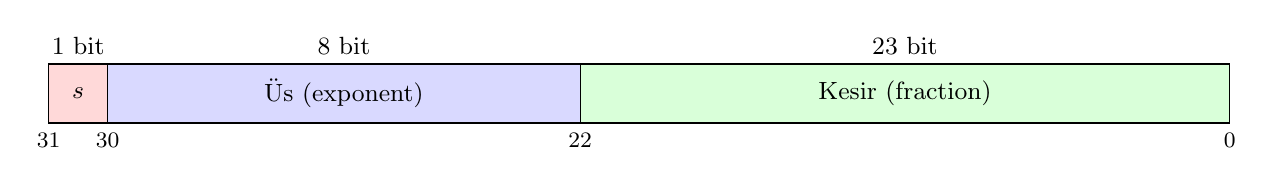
\begin{tikzpicture}[scale=0.75, every node/.style={font=\small}]
  % İşaret biti
  \draw[fill=red!15] (0,0) rectangle (1,1);
  \node at (0.5, 0.5) {$s$};
  \node[above] at (0.5, 1) {1 bit};
  % Üs alanı
  \draw[fill=blue!15] (1,0) rectangle (9,1);
  \node at (5, 0.5) {Üs (exponent)};
  \node[above] at (5, 1) {8 bit};
  % Kesir alanı
  \draw[fill=green!15] (9,0) rectangle (20,1);
  \node at (14.5, 0.5) {Kesir (fraction)};
  \node[above] at (14.5, 1) {23 bit};
  % Bit numaraları
  \node[below, font=\footnotesize] at (0, 0) {31};
  \node[below, font=\footnotesize] at (1, 0) {30};
  \node[below, font=\footnotesize] at (9, 0) {22};
  \node[below, font=\footnotesize] at (20, 0) {0};
\end{tikzpicture}
\caption{IEEE 754 tek duyarlı kayan nokta biçimi}
\label{fig:ieee754-tek}
\end{figure}

Sayının değeri şu formülle hesaplanır:
\begin{equation}
\text{değer} = (-1)^s \times 1{,}f \times 2^{(e - 127)}
\label{eq:ieee754}
\end{equation}
Burada $s$ işaret biti, $e$ üs alanının işaretsiz tam sayı değeri ve $f$ kesir alanıdır. Üs alanında 127 \textbf{kaydırması}\index{üs kaydırması} (İngilizcesi: \textit{bias}) kullanılır: saklanan $e$ değerinden 127 çıkarılarak gerçek üs elde edilir. $e = 127$ ise gerçek üs $0$, $e = 130$ ise gerçek üs $+3$, $e = 124$ ise gerçek üs $-3$ olur.

Kesir alanının solunda örtük bir ``$1,$'' bulunur (normalleştirilmiş sayılarda); bu sayede 23 bitlik kesir alanı aslında 24 bitlik bir doğruluk sağlar.

\subsection{IEEE 754 Duyarlık Düzeyleri}
\label{sec:ekA-ieee754-duzeyler}

IEEE~754 standardı farklı duyarlık düzeyleri tanımlar. Dört temel biçim Şekil~\ref{fig:ieee754-tum}'de karşılaştırmalı olarak gösterilmiştir; tüm biçimlerde yapı aynıdır (işaret $+$ üs $+$ kesir), yalnızca alan genişlikleri farklıdır.

\begin{figure}[H]
\centering
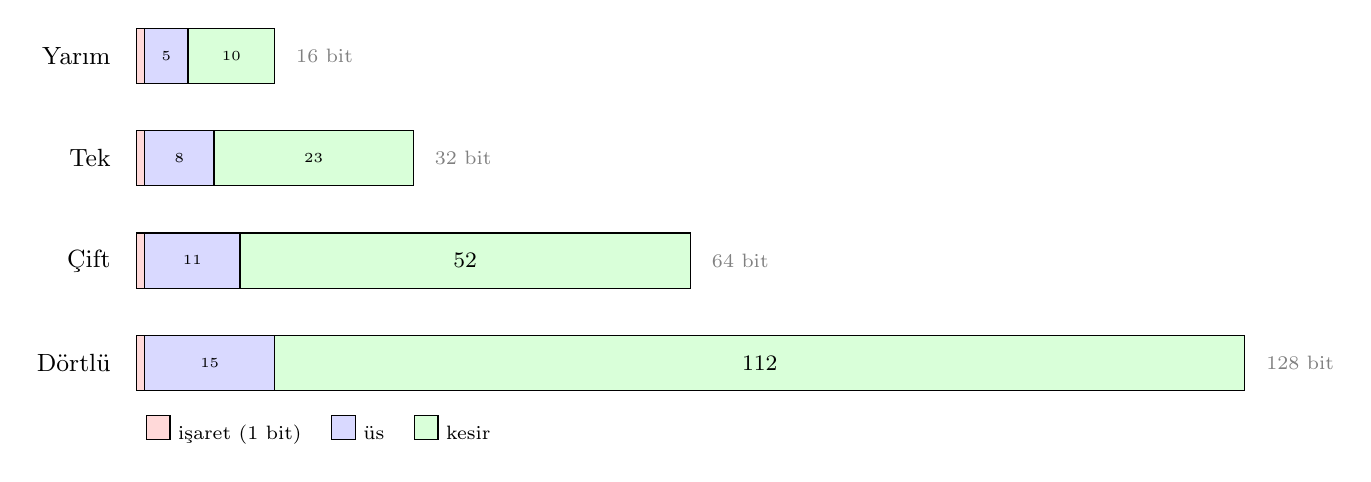
\begin{tikzpicture}[every node/.style={font=\footnotesize}]
  % Orantılı genişlik: 1 bit = 0.11 TikZ birimi (128 bit → ~14 cm)
  \def\bpu{0.11}
  \def\barh{0.7}
  \def\gap{1.3}

  % ---- Yarım (binary16): 1 + 5 + 10 = 16 bit ----
  \pgfmathsetmacro{\yrow}{3*\gap}
  \pgfmathsetmacro{\ysign}{1*\bpu}
  \pgfmathsetmacro{\yexp}{5*\bpu}
  \pgfmathsetmacro{\yfrac}{10*\bpu}
  \pgfmathsetmacro{\ytotal}{16*\bpu}
  \node[anchor=east, font=\small] at (-0.2, \yrow+\barh/2) {Yarım};
  \draw[fill=red!15]   (0,\yrow) rectangle (\ysign, \yrow+\barh);
  \draw[fill=blue!15]  (\ysign,\yrow) rectangle ({\ysign+\yexp}, \yrow+\barh);
  \draw[fill=green!15] ({\ysign+\yexp},\yrow) rectangle (\ytotal, \yrow+\barh);
  \node[font=\tiny] at ({\ysign+\yexp/2}, \yrow+\barh/2) {5};
  \node[font=\tiny] at ({\ysign+\yexp+\yfrac/2}, \yrow+\barh/2) {10};
  \node[anchor=west, font=\scriptsize, gray] at ({\ytotal+0.15}, \yrow+\barh/2) {16 bit};

  % ---- Tek (binary32): 1 + 8 + 23 = 32 bit ----
  \pgfmathsetmacro{\trow}{2*\gap}
  \pgfmathsetmacro{\tsign}{1*\bpu}
  \pgfmathsetmacro{\texp}{8*\bpu}
  \pgfmathsetmacro{\tfrac}{23*\bpu}
  \pgfmathsetmacro{\ttotal}{32*\bpu}
  \node[anchor=east, font=\small] at (-0.2, \trow+\barh/2) {Tek};
  \draw[fill=red!15]   (0,\trow) rectangle (\tsign, \trow+\barh);
  \draw[fill=blue!15]  (\tsign,\trow) rectangle ({\tsign+\texp}, \trow+\barh);
  \draw[fill=green!15] ({\tsign+\texp},\trow) rectangle (\ttotal, \trow+\barh);
  \node[font=\tiny] at ({\tsign+\texp/2}, \trow+\barh/2) {8};
  \node[font=\tiny] at ({\tsign+\texp+\tfrac/2}, \trow+\barh/2) {23};
  \node[anchor=west, font=\scriptsize, gray] at ({\ttotal+0.15}, \trow+\barh/2) {32 bit};

  % ---- Çift (binary64): 1 + 11 + 52 = 64 bit ----
  \pgfmathsetmacro{\crow}{1*\gap}
  \pgfmathsetmacro{\csign}{1*\bpu}
  \pgfmathsetmacro{\cexp}{11*\bpu}
  \pgfmathsetmacro{\cfrac}{52*\bpu}
  \pgfmathsetmacro{\ctotal}{64*\bpu}
  \node[anchor=east, font=\small] at (-0.2, \crow+\barh/2) {Çift};
  \draw[fill=red!15]   (0,\crow) rectangle (\csign, \crow+\barh);
  \draw[fill=blue!15]  (\csign,\crow) rectangle ({\csign+\cexp}, \crow+\barh);
  \draw[fill=green!15] ({\csign+\cexp},\crow) rectangle (\ctotal, \crow+\barh);
  \node[font=\tiny] at ({\csign+\cexp/2}, \crow+\barh/2) {11};
  \node at ({\csign+\cexp+\cfrac/2}, \crow+\barh/2) {52};
  \node[anchor=west, font=\scriptsize, gray] at ({\ctotal+0.15}, \crow+\barh/2) {64 bit};

  % ---- Dörtlü (binary128): 1 + 15 + 112 = 128 bit ----
  \pgfmathsetmacro{\drow}{0}
  \pgfmathsetmacro{\dsign}{1*\bpu}
  \pgfmathsetmacro{\dexp}{15*\bpu}
  \pgfmathsetmacro{\dfrac}{112*\bpu}
  \pgfmathsetmacro{\dtotal}{128*\bpu}
  \node[anchor=east, font=\small] at (-0.2, \drow+\barh/2) {Dörtlü};
  \draw[fill=red!15]   (0,\drow) rectangle (\dsign, \drow+\barh);
  \draw[fill=blue!15]  (\dsign,\drow) rectangle ({\dsign+\dexp}, \drow+\barh);
  \draw[fill=green!15] ({\dsign+\dexp},\drow) rectangle (\dtotal, \drow+\barh);
  \node[font=\tiny] at ({\dsign+\dexp/2}, \drow+\barh/2) {15};
  \node at ({\dsign+\dexp+\dfrac/2}, \drow+\barh/2) {112};
  \node[anchor=west, font=\scriptsize, gray] at ({\dtotal+0.15}, \drow+\barh/2) {128 bit};

  % Renk açıklaması
  \node[anchor=west, font=\scriptsize] at (0, -0.5) {%
    \tikz{\draw[fill=red!15] (0,0) rectangle (0.3,0.3);} işaret (1 bit)
    \quad
    \tikz{\draw[fill=blue!15] (0,0) rectangle (0.3,0.3);} üs
    \quad
    \tikz{\draw[fill=green!15] (0,0) rectangle (0.3,0.3);} kesir};
\end{tikzpicture}
\caption{IEEE 754 kayan nokta biçimlerinin karşılaştırması}
\label{fig:ieee754-tum}
\end{figure}

\textbf{Yarım duyarlı (16 bit):} 2008 yılında IEEE~754 standardına eklenen bu biçim (binary16), derin öğrenme ve grafik uygulamalarında bellek ve bant genişliğinden tasarruf etmek için kullanılır. Yalnızca $\sim$3 ondalık basamak doğruluk sağladığı için genel amaçlı hesaplamalar için uygun değildir.

\textbf{Çift duyarlı (64 bit):} Çoğu programlama dilinde varsayılan kayan nokta türüdür. $\sim$16 basamak doğruluk sağlar ve bilimsel hesaplamaların büyük çoğunluğu için yeterlidir.

\textbf{Dörtlü duyarlı (128 bit):} $\sim$34 basamak doğruluk sağlar; astronomik hesaplamalar ve çok hassas sayısal çözücüler gibi özel alanlarda kullanılır. Çoğu işlemci donanımda desteklemez; yazılımla gerçekleştirilir.

Dört duyarlık düzeyinin alan genişlikleri, üs aralıkları ve gösterim kapasiteleri Tablo~\ref{tab:ieee754-karsilastirma}'da özetlenmiştir.

\begin{table}[H]
\centering
\caption{IEEE 754 duyarlık düzeylerinin karşılaştırması}
\label{tab:ieee754-karsilastirma}
\small
\begin{tabular}{lcccc}
\toprule
\textbf{Özellik} & \textbf{Yarım} & \textbf{Tek} & \textbf{Çift} & \textbf{Dörtlü} \\
\midrule
Toplam bit sayısı       & 16     & 32     & 64      & 128 \\
İşaret biti             & 1      & 1      & 1       & 1 \\
Üs alanı                & 5 bit  & 8 bit  & 11 bit  & 15 bit \\
Kesir alanı             & 10 bit & 23 bit & 52 bit  & 112 bit \\
Üs kaydırması           & 15     & 127    & 1023    & 16383 \\
Üs aralığı              & $-14$ -- $+15$ & $-126$ -- $+127$ & $-1022$ -- $+1023$ & $-16382$ -- $+16383$ \\
Ondalık doğruluk        & $\sim$3    & $\sim$7    & $\sim$16   & $\sim$34 \\
En küçük normalleşt.    & $\sim 6{,}1 \times 10^{-5}$ & $\sim 1{,}2 \times 10^{-38}$ & $\sim 2{,}2 \times 10^{-308}$ & $\sim 3{,}4 \times 10^{-4932}$ \\
En büyük sonlu          & $\sim 6{,}6 \times 10^{4}$  & $\sim 3{,}4 \times 10^{38}$  & $\sim 1{,}8 \times 10^{308}$  & $\sim 1{,}2 \times 10^{4932}$ \\
\bottomrule
\end{tabular}
\end{table}

\subsection{Özel Değerler}
\label{sec:ekA-ieee754-ozel}

IEEE~754 standardı, olağan sayıların yanı sıra birkaç özel durumu da tanımlar. Tablo~\ref{tab:ieee754-ozel}'de üs ve kesir alanlarının özel kombinasyonlarına karşılık gelen değerler listelenmiştir.

\begin{table}[H]
\centering
\caption{IEEE 754 özel değerler (tek duyarlı)}
\label{tab:ieee754-ozel}
\begin{tabular}{ccl}
\toprule
\textbf{Üs ($e$)} & \textbf{Kesir ($f$)} & \textbf{Gösterilen değer} \\
\midrule
0       & 0       & $\pm 0$ (işaret bitine bağlı) \\
0       & $\neq 0$  & Denormalize sayı: $(-1)^s \times 0{,}f \times 2^{-126}$ \\
1--254  & herhangi  & Normalleştirilmiş sayı: $(-1)^s \times 1{,}f \times 2^{(e-127)}$ \\
255     & 0       & $\pm \infty$ (sonsuz) \\
255     & $\neq 0$  & NaN (sayı değil — \textit{Not a Number}) \\
\bottomrule
\end{tabular}
\end{table}

Sonsuz ($\infty$) değeri, sıfıra bölme gibi işlemlerin sonucu olarak ortaya çıkar. NaN ise $0/0$ veya $\sqrt{-1}$ gibi tanımsız işlemlerin sonucudur. Bu özel değerler sayesinde program çökmek yerine hesaplamaya devam edebilir ve hata daha sonra tespit edilebilir.

\begin{ornek}[A.24]
$-6{,}625$ sayısını IEEE~754 tek duyarlı biçimde gösterin.

\textbf{Çözüm:}

\textit{Adım 1 (İşaret biti):} Sayı negatif olduğu için $s = 1$.

\textit{Adım 2 (İkilik tabana çevirme):} $6 = (110)_2$; kesir kısmı: $0{,}625 = 0{,}5 + 0{,}125 = 2^{-1} + 2^{-3} = (0{,}101)_2$. Dolayısıyla $6{,}625 = (110{,}101)_2$.

\textit{Adım 3 (Normalleştirme):} Noktayı sola kaydırarak $1{,}10101 \times 2^2$ elde edilir.

\textit{Adım 4 (Üs hesabı):} Gerçek üs $= 2$; saklanan üs $= 2 + 127 = 129 = (10000001)_2$.

\textit{Adım 5 (Kesir alanı):} Örtük 1 atılır, kalan $10101$ sağdan sıfırlarla 23 bite tamamlanır: $10101000000000000000000$.

Sonuç:
\[
\underbrace{1}_{s}\;\underbrace{10000001}_{e=129}\;\underbrace{10101000000000000000000}_{f} = \texttt{C0D40000}_{16}
\]
\end{ornek}

\begin{ornek}[A.25]
IEEE~754 tek duyarlı biçimde saklanan \texttt{41C80000}$_{16}$ değerinin onluk tabandaki karşılığını bulun.

\textbf{Çözüm:}

Onaltılık değeri ikilik tabana açalım:
\[
\texttt{41C80000}_{16} = 0\;10000011\;10010000000000000000000
\]
İşaret: $s = 0$ (pozitif). Üs: $e = (10000011)_2 = 131$; gerçek üs $= 131 - 127 = 4$. Kesir: $f = 10010\ldots$; örtük 1 ile: $1{,}1001$. Değer: $1{,}1001 \times 2^4 = 11001{,}0 = 16 + 8 + 1 = 25{,}0$. Sonuç: $+25{,}0$.
\end{ornek}

\begin{ornek}[A.26]
IEEE~754 tek duyarlı biçimde $0{,}1$ sayısını gösterin. Geri dönüşümde tam olarak $0{,}1$ elde edilir mi?

\textbf{Çözüm:}

$0{,}1$ sayısının ikilik tabandaki açılımı sonsuz yinelenen bir kesirdir:
\[
0{,}1_{10} = 0{,}0\overline{0011}\;0\overline{0011}\ldots_2
\]
Normalleştirme: $1{,}\overline{1001}\;1001\ldots \times 2^{-4}$. İşaret: $s = 0$. Üs: $-4 + 127 = 123 = (01111011)_2$. Kesir alanına 23 bit sığdırılır ve yuvarlanır. Sonuç:
\[
0\;01111011\;10011001100110011001101 = \texttt{3DCCCCCD}_{16}
\]
Geri dönüşümde elde edilen değer tam olarak $0{,}1$ değildir; yaklaşık $0{,}100000001490\ldots$ olur. Bu fark, kayan nokta aritmetiğinde \textbf{yuvarlama hatası}\index{yuvarlama hatası} olarak bilinir ve bilgisayar aritmetiğinin temel sınırlamalarından biridir.
\end{ornek}


% =====================================================
% A.7 Yanılgılar ve Tuzaklar
% =====================================================
\section{Yanılgılar ve Tuzaklar}
\label{sec:yanilgilar-tuzaklar-sayi-sistemleri}

Sayı sistemleri ve kodlama yöntemleri ilk bakışta mekanik kurallar bütünü gibi görünse de uygulamada sürpriz hatalar doğuran pek çok yanılgı ve tuzak barındırır\index{yanılgılar ve tuzaklar}. Sezginin yanıltıcı olduğu bu noktalarda küçük bir kavram kargaşası, yazılım hatalarına ya da donanım tasarımında beklenmeyen davranışlara yol açabilir.

\yanilgi{İkiye tümleyende en yüksek değerli bit yalnızca işaret bitidir ve farklı işlenir}
$n$-bitlik ikiye tümleyen gösteriminde en yüksek değerli bit, $-2^{n-1}$ ağırlığına sahip sıradan bir bit konumudur; geri kalan bitler ise $+2^{n-2}, +2^{n-3}, \ldots, +2^0$ ağırlıklarıyla katkıda bulunur. Toplama ve çıkarma işlemleri, bu bit için özel bir kural gerektirmeksizin modüler aritmetikle gerçekleştirilir. Örneğin 4-bitlik gösterimde $1101_2$ değeri $-3$'tür: $-8 + 4 + 0 + 1 = -3$. Donanım toplayıcısı bu sayıyı diğerlerinden farklı biçimde işlemez; tüm bitler aynı devre kurallarına tabidir. ``İşaret biti ayrı hesaplanır'' yanılgısı, konunun tersine tümleyen ve işaret-büyüklük gösterimleriyle birlikte öğrenilmesinden kaynaklanır; oysa ikiye tümleyene geçilince bu ayrım ortadan kalkar.

\tuzak{İşaretli ve işaretsiz karşılaştırmayı karıştırmak}
C ve C++ dillerinde \texttt{int} ile \texttt{unsigned int} türleri aynı bit kalıbını farklı yorumlar. İki değer karşılaştırıldığında derleyici, kurallar gereği \texttt{int} tarafını \texttt{unsigned}'a dönüştürür. Bu durumda $-1$ değeri, 32-bitlik gösterimde $2^{32}-1 = 4\,294\,967\,295$ olarak yorumlanır ve karşılaştırma ``\texttt{-1 > 1}'' ifadesi beklenmedik biçimde doğru sonuç verir. Döngülerde \texttt{i >= 0} koşuluyla kullanılan işaretsiz sayaç hiç sonlanmaz; çünkü işaretsiz tamsayılar her zaman sıfırdan büyük ya da eşittir. Bu tuzağa düşmemek için karşılaştırma operandlarının türlerini açıkça eşleştirmek gerekir.

\yanilgi{ASCII Türkçe karakterleri kapsar}
ASCII, 7~bit ile yalnızca 128 karakter tanımlar; bunlar temel Latin harfleri, rakamlar ve noktalama işaretleridir. Ğ, ğ, İ, ı, Ö, ö, Ş, ş, Ü, ü gibi Türkçe karakterler bu kümede yer almaz. Bu karakterleri aktarmak için ISO~8859-9 (Latin-5) ya da UTF-8 kodlaması gereklidir. ``Bilgisayar zaten ASCII kullanıyorsa Türkçe de çalışır'' yanılgısı, tarihsel olarak Türkçe metin dosyalarında veri bozulmasına ve platformlar arası uyumsuzluğa yol açmıştır. UTF-8, ASCII ile tam geriye dönük uyumlu olduğundan ve tüm Unicode karakterlerini desteklediğinden çağdaş sistemlerde tercih edilen standarttır.

\tuzak{Kayan nokta sayılarını \texttt{==} ile karşılaştırmak}
İkili gösterim, $0{,}1$ gibi pek çok onluk kesri tam olarak ifade edemez; bu nedenle $0{,}1 + 0{,}2$ işleminin sonucu IEEE~754 tek duyarlıda tam olarak $0{,}3$ değil $0{,}30000001192\ldots$ olur. Eşitlik karşılaştırması iki kayan nokta sayısının bit bit örtüşmesini arar; art arda yapılan hesaplar kümülâtif yuvarlama hatası biriktirdiğinden aynı matematiksel değer farklı bit kalıplarına dönüşebilir. Doğru yaklaşım $|a - b| < \varepsilon$ biçiminde bir hata payı denetimidir; burada $\varepsilon$ değeri uygulamaya özgü bir tolerans sınırıdır. Özellikle döngü sayacı ve durdurma koşulu olarak kayan nokta karşılaştırması kullanmak ciddi hataya kapı aralar.

\yanilgi{Kayan nokta aritmetiği sınırsız hassasiyet sunar}
IEEE~754 tek duyarlı biçimde kesir alanı yalnızca 23 bit genişliğindedir; bu, yaklaşık 7~onluk basamak duyarlığa karşılık gelir. Çift duyarlıda bu değer 15--16~basamağa çıkar, ancak yine de sonsuza değil. Bilimsel hesaplamalarda art arda gerçekleştirilen toplama ve çıkarma işlemleri bağıl hata büyüklüğünü artırabilir (felaket iptali); döngüsel toplama yöntemi (Kahan toplamı) bu hatayı hafifletir. Yapay zeka uygulamalarında kullanılan yarım duyarlı (16~bit) biçim ise yalnızca 3~onluk basamak hassasiyet sağlar. ``Kayan nokta kesindir, tamsayı gibi güvenilir'' anlayışı, finans ve ölçüm yazılımlarında ciddi hatalara neden olmuştur.

\tuzak{BCD ile ikilik gösterimi karıştırmak}
BCD'de her onluk basamak bağımsız olarak 4~bit ile kodlanır: $29_{10}$ değeri BCD'de \texttt{0010 1001} olurken ikilik gösterimde \texttt{00011101} olur. Bu iki gösterim görünüşte benzer bit dizileri üretebilir, ancak değerleri farklıdır. BCD toplamasında her 4-bitlik grup için kural dışı durum denetimi (sonuç 9'u aşıyorsa 6 eklenir) gereklidir; standart ikilik toplayıcı bu düzeltmeyi otomatik yapmaz. Donanım ve yazılım arasında veri aktarımında kodlama biçiminin belgelenmemesi, BCD ile ikilik verinin birbirinin yerine yorumlanmasına ve yanlış sayı gösterimine yol açar.

\tuzak{Negatif ikilik sayı çevrilirken mutlak değer adımını atlamak}
Bir onluk negatif sayıyı ikiye tümleyen gösterimine dönüştürmenin klasik yöntemi şudur: (1) sayının mutlak değerini ikilik tabanda yaz, (2) tüm bitleri tersle, (3) sonuca 1 ekle. Yaygın hata, mutlak değer alınmadan doğrudan negatif sayının basamakları üzerinden işlem yapmaktır. Örneğin $-5$'i 4~bitte göstermek için önce $5 = 0101_2$, sonra tersle $1010_2$, son olarak $1 + 1010_2 = 1011_2$ adımları izlenir. ``Eksi işaretini kor, kalanı çevir'' yaklaşımı hatalı sonuç verir ve doğrulama yapılmadan donanım tasarımına taşındığında zorlu hata ayıklama süreçlerine kapı aralar.

\yanilgi{Onaltılık gösterim yalnızca bir yazım biçimidir, 16 tabanıyla ilgisi yoktur}
Onaltılık (hex) gösterim, 16 tabanlı bir sayı sistemidir: her basamak $0$'dan $\text{F}$'ye kadar 16 farklı değer alır ve $n$. konumdaki basamak $16^n$ ile ağırlıklandırılır. ``Hex yalnızca ikilik bitlerin okunabilir biçimde gösterilmesidir'' düşüncesi bu sistemi indirger. Onaltılık basamaklar ikilik gruplarla doğrudan eşleştiğinden (her hex basamağı 4~bit) dönüşüm kolaydır; ancak bu kolaylık, hex'in bağımsız bir sayı sistemi olduğu gerçeğini değiştirmez. Aritmetik işlemler hex basamaklarına doğrudan uygulanabilir: $\text{A}_{16} + \text{B}_{16} = \text{15}_{16}$ hesabı ikilik tabana başvurmadan yapılabilir.

% =====================================================
\section*{Özet}
\addcontentsline{toc}{section}{Özet}

Bu ekte bilgisayar mimarisinin temelini oluşturan sayı sistemleri ve kodlama yöntemleri ele alındı. Temel kavramlar şöyle özetlenebilir:

\begin{itemize}
\item İkilik taban, bilgisayarların doğal dilidir. Taban dönüşümleri, her basamağın taban kuvvetleriyle çarpılıp toplanması ilkesine dayanır (Denklem~\ref{eq:taban-donusum}).

\item Sekizlik ve onaltılık tabanlar, uzun ikilik dizileri sırasıyla 3'erli ve 4'erli gruplara ayırarak okunabilirliği artırır.

\item İşaretli sayılar arasında \emph{ikiye tümleyen} yöntemi, tek sıfır değeri ve basit donanım gerçekleştirimi sayesinde günümüz işlemcilerinde standart olmuştur. Taşma, aynı işaretli iki sayının toplamında sonuç aralık dışına çıktığında oluşur; farklı işaretli sayıların toplamında oluşmaz.

\item Gray kodu, ardışık sayılar arasında yalnızca tek bitin değişmesini garanti ederek geçiş hatalarını önler. BCD gösterimi ise her onluk basamağı ayrı 4 bitle kodlar.

\item ASCII, 7~bitlik kodlamayla 128 karakter tanımlar. Unicode ve UTF-8 ise değişken uzunluklu kodlamayla dünyadaki tüm yazı sistemlerini kapsar.

\item IEEE~754 kayan nokta standardı; işaret, üs ve kesir alanlarıyla kesirli sayıları gösterir. Tek duyarlı (32~bit) ve çift duyarlı (64~bit) biçimler en yaygın kullanılanlardır. Kayan nokta aritmetiğinin ayrıntıları Bölüm~\ref{chap:aritmetik}'te ele alınmaktadır.
\end{itemize}


% =====================================================
\section*{Alıştırmalar}
\addcontentsline{toc}{section}{Alıştırmalar}
\label{sec:ekA-alistirmalar}

\begin{alistirma}[\kolay]
$(54)_{10}$ sayısını ikilik, sekizlik ve onaltılık tabanda yazın.
\end{alistirma}

\begin{alistirma}[\kolay]
İkilik tabandaki $(11001110)_2$ sayısını onluk, sekizlik ve onaltılık tabanda yazın.
\end{alistirma}

\begin{alistirma}[\kolay]
Aşağıdaki 8 bitlik ikiye tümleyen sayıların onluk tabandaki karşılıklarını bulun: (a)~$01100100$, (b)~$10110011$, (c)~$11111111$, (d)~$10000000$.
\end{alistirma}

\begin{alistirma}[\kolay]
ASCII tablosunu kullanarak ``RISC-V'' dizgisinin her bir karakterinin onaltılık kodunu yazın.
\end{alistirma}

\begin{alistirma}[\kolay]
$(-23)_{10}$ sayısının 8 bitlik ikiye tümleyen gösterimini bulun. Sonucu onaltılık tabanda da ifade edin.
\end{alistirma}

\begin{alistirma}[\kolay]
3 bitlik Gray kodunu kullanarak $(5)_{10}$ sayısının Gray kodu karşılığını bulun.
\end{alistirma}

\begin{alistirma}[\orta]
8 bitlik ikiye tümleyen düzeninde aşağıdaki toplama işlemlerini yapın ve taşma olup olmadığını belirleyin: (a)~$64 + 53$, (b)~$(-80) + (-60)$, (c)~$100 + (-75)$.
\end{alistirma}

\begin{alistirma}[\orta]
4 bitlik bir ikiye tümleyen sisteminde gösterilebilecek en küçük ve en büyük tam sayıları belirleyin. 16 bit için aynı hesabı yineleyin.
\end{alistirma}

\begin{alistirma}[\orta]
$12{,}375$ sayısını IEEE~754 tek duyarlı kayan nokta biçiminde gösterin. Sonucu onaltılık tabanda da ifade edin.
\end{alistirma}

\begin{alistirma}[\orta]
IEEE~754 tek duyarlı biçimde saklanan \texttt{C1480000}$_{16}$ değerinin onluk tabandaki karşılığını bulun.
\end{alistirma}

\begin{alistirma}[\orta]
BCD düzeninde $49 + 38$ işlemini yapın. 4 bitlik her grubun sonucunu ayrı ayrı gösterin ve gerekli düzeltme adımlarını açıklayın.
\end{alistirma}

\begin{alistirma}[\orta]
``Öğüz'' kelimesinin UTF-8 kodlamasını onaltılık tabanda yazın. Her karakter için kaç bayt kullanıldığını belirtin. (İpucu: Ö = U+00D6, ğ = U+011F, ü = U+00FC, z = U+007A)
\end{alistirma}

\begin{alistirma}[\orta]
8 bitlik $01011010$ sayısını aşağıdaki her yöntemle yorumlayın ve onluk tabandaki karşılığını verin: (a)~işaretsiz, (b)~ayrı işaret biti, (c)~bire tümleyen, (d)~ikiye tümleyen.
\end{alistirma}

\begin{alistirma}[\orta]
$(-19)_{10}$ sayısını 8 bitlik ikiye tümleyen biçiminde bulun; ardından 16 bite işaretle genişletme uygulayın. Her iki gösterimin de onluk tabandaki değerinin aynı olduğunu doğrulayın.
\end{alistirma}

\begin{alistirma}[\zor]
IEEE~754 tek duyarlı biçimde $+\infty$, $-0$ ve NaN değerlerinin ikilik tabandaki gösterimlerini yazın.
\end{alistirma}

\begin{alistirma}[\zor]
IEEE~754 tek duyarlı biçimde gösterilebilecek, sıfırdan büyük en küçük normalleştirilmiş sayıyı ve en küçük denormalize sayıyı bulun. Bu iki değer arasındaki farkı açıklayın.
\end{alistirma}

\begin{alistirma}[\zor]
Birçok programlama dilinde \texttt{0.1 + 0.2 != 0.3} ifadesi doğru (true) sonuç verir. IEEE~754 tek duyarlı aritmetiğini kullanarak bu durumu açıklayın. $0{,}1$, $0{,}2$ ve $0{,}3$ sayılarının kayan nokta gösterimlerini karşılaştırın.
\end{alistirma}

\begin{alistirma}[\zor]
$n$ bitlik ikiye tümleyen düzeninde $-2^{n-1}$ sayısının ikiye tümleyenini almaya çalışın. Sonuç nedir ve bu neden bir sorun oluşturur?
\end{alistirma}
